%%%%%%%%%%%%%%%%%%%%%%%%%%%%%%%%%%%%%%%%%%%%%%%%%%%%%%%%%%%%%%%%%%%%%%%%%%%%%%%%%%%%%%%%%%%%%%%%
%
% CS484 Written Question Template
%
% Acknowledgements:
% The original code is written by Prof. James Tompkin (james_tompkin@brown.edu).
% The second version is revised by Prof. Min H. Kim (minhkim@kaist.ac.kr).
%
% This is a LaTeX document. LaTeX is a markup language for producing 
% documents. Your task is to fill out this document, then to compile 
% it into a PDF document. 
%
% 
% TO COMPILE:
% > pdflatex thisfile.tex
%
% If you do not have LaTeX and need a LaTeX distribution:
% - Personal laptops (all common OS): www.latex-project.org/get/
% - We recommend latex compiler miktex (https://miktex.org/) for windows,
%   macTex (http://www.tug.org/mactex/) for macOS users.
%   And TeXstudio(http://www.texstudio.org/) for latex editor.
%   You should install both compiler and editor for editing latex.
%   The another option is Overleaf (https://www.overleaf.com/) which is 
%   an online latex editor.
%
% If you need help with LaTeX, please come to office hours. 
% Or, there is plenty of help online:
% https://en.wikibooks.org/wiki/LaTeX
%
% Good luck!
% Min and the CS484 staff
%
%%%%%%%%%%%%%%%%%%%%%%%%%%%%%%%%%%%%%%%%%%%%%%%%%%%%%%%%%%%%%%%%%%%%%%%%%%%%%%%%%%%%%%%%%%%%%%%%
%
% How to include two graphics on the same line:
% 
% \includegraphics[width=0.49\linewidth]{yourgraphic1.png}
% \includegraphics[width=0.49\linewidth]{yourgraphic2.png}
%
% How to include equations:
%
% \begin{equation}
% y = mx+c
% \end{equation}
% 
%%%%%%%%%%%%%%%%%%%%%%%%%%%%%%%%%%%%%%%%%%%%%%%%%%%%%%%%%%%%%%%%%%%%%%%%%%%%%%%%%%%%%%%%%%%%%%%%

\documentclass[11pt]{article}

\usepackage[english]{babel}
\usepackage[utf8]{inputenc}
\usepackage[colorlinks = true,
            linkcolor = blue,
            urlcolor  = blue]{hyperref}
\usepackage[a4paper,margin=1.5in]{geometry}
\usepackage{stackengine,graphicx}
\usepackage{fancyhdr}
\setlength{\headheight}{15pt}
\usepackage{microtype}
\usepackage{times}
\usepackage{booktabs}

% From https://ctan.org/pkg/matlab-prettifier
\usepackage[numbered,framed]{matlab-prettifier}

\frenchspacing
\setlength{\parindent}{0cm} % Default is 15pt.
\setlength{\parskip}{0.3cm plus1mm minus1mm}

\pagestyle{fancy}
\fancyhf{}
\lhead{Project Writeup}
\rhead{CS 484}
\rfoot{\thepage}

\date{}

\title{\vspace{-1cm}Homework 4 Writeup}


\begin{document}
\maketitle
\vspace{-3cm}
\thispagestyle{fancy}

\section*{Instructions}
\begin{itemize}
  \item Describe any interesting decisions you made to write your algorithm.
  \item Show and discuss the results of your algorithm.
  \item Feel free to include code snippets, images, and equations.
  \item Use as many pages as you need, but err on the short side If you feel you only need to write a short amount to meet the brief, th
  
  \item \textbf{Please make this document anonymous.}
\end{itemize}

\section*{In the beginning...}

There are interesting points.\\
- Gradient by filtering.\\
- Gaussian filtering before get descriptors.\\
- Non-maxima supression
 
\section*{Interesting Implementation Detail}


For calculating image gradients Ix and Iy, I use the filter below.
\begin{lstlisting}[style=Matlab-editor]
gy = [0 1 0;0 0 0;0 -1 0];
gx = gy';
ix = imfilter(image, gx);
iy = imfilter(image, gy);
\end{lstlisting}

Before start the get descriptors function, I filter the image with gaussian filter. This improve the accuracy (on first 100 confident) of ND. Please refer to the Result section. 
\begin{lstlisting}[style=Matlab-editor]
image = imfilter(image, image_gaussian);
\end{lstlisting}

While doing "get interest points.m", I use the matlab function colfilt(). The function extract the local maximum value of the cornerness. This will make feature points evenly distributed.
\begin{lstlisting}[style=Matlab-editor]
Cmax = colfilt(C, [descriptor window image width descriptor window image width], 'sliding', @max);
C = C.*(C == Cmax);
\end{lstlisting}

\newpage
\section*{A Result}

When using normalized patches (NP) for feature descriptors:
\begin{enumerate}
    \item Notre Dame de Paris (Figure~\ref{fig:result1})\\
    Accuracy:  48.5 (on all 167 submitted matches)\\
    Accuracy:  62 (on first 100 matches sorted by decreasing confidence)
    \item Mount Rushmore (Figure~\ref{fig:result2})\\
    Accuracy:  81 (on all 221 submitted matches)\\
    Accuracy:  88 (on first 100 matches sorted by decreasing confidence)
    \item Gaudi's Episcopal Palace (Figure~\ref{fig:result3})\\
    Accuracy:  0 (on all 11 submitted matches)\\ 
    Accuracy:  0 (on first 100 matches sorted by decreasing confidence)
\end{enumerate}


When using SIFT-like for feature descriptors:
\begin{enumerate}
    \item Notre Dame de Paris (Figure~\ref{fig:result4})\\
    Accuracy:  85.34 (on all 116 submitted matches)\\
    Accuracy:  90 (on first 100 matches sorted by decreasing confidence)
    \item Mount Rushmore (Figure~\ref{fig:result5})\\
    Accuracy:  89.41 (on all 236 submitted matches)\\
    Accuracy:  97 (on first 100 matches sorted by decreasing confidence)
    \item Gaudi's Episcopal Palace (Figure~\ref{fig:result6})\\
    Accuracy:  0 (on all 5 submitted matches)\\ 
    Accuracy:  0 (on first 100 matches sorted by decreasing confidence)
\end{enumerate}


When using SIFT-like for feature descriptors without gaussian filtered image:
\begin{enumerate}
    \item Notre Dame de Paris (Figure~\ref{fig:result7})\\
    Accuracy:  92.45 (on all 53 submitted matches)\\
    Accuracy:  49 (on first 100 matches sorted by decreasing confidence)
    \item Mount Rushmore (Figure~\ref{fig:result8})\\
    Accuracy:  95.35 (on all 129 submitted matches)\\
    Accuracy:  98 (on first 100 matches sorted by decreasing confidence)
    \item Gaudi's Episcopal Palace (Figure~\ref{fig:result9})\\
    Accuracy:  NaN (on all 0 submitted matches)\\
    Accuracy:  0 (on first 100 matches sorted by decreasing confidence)
\end{enumerate}


\begin{figure}[h]
    \centering
    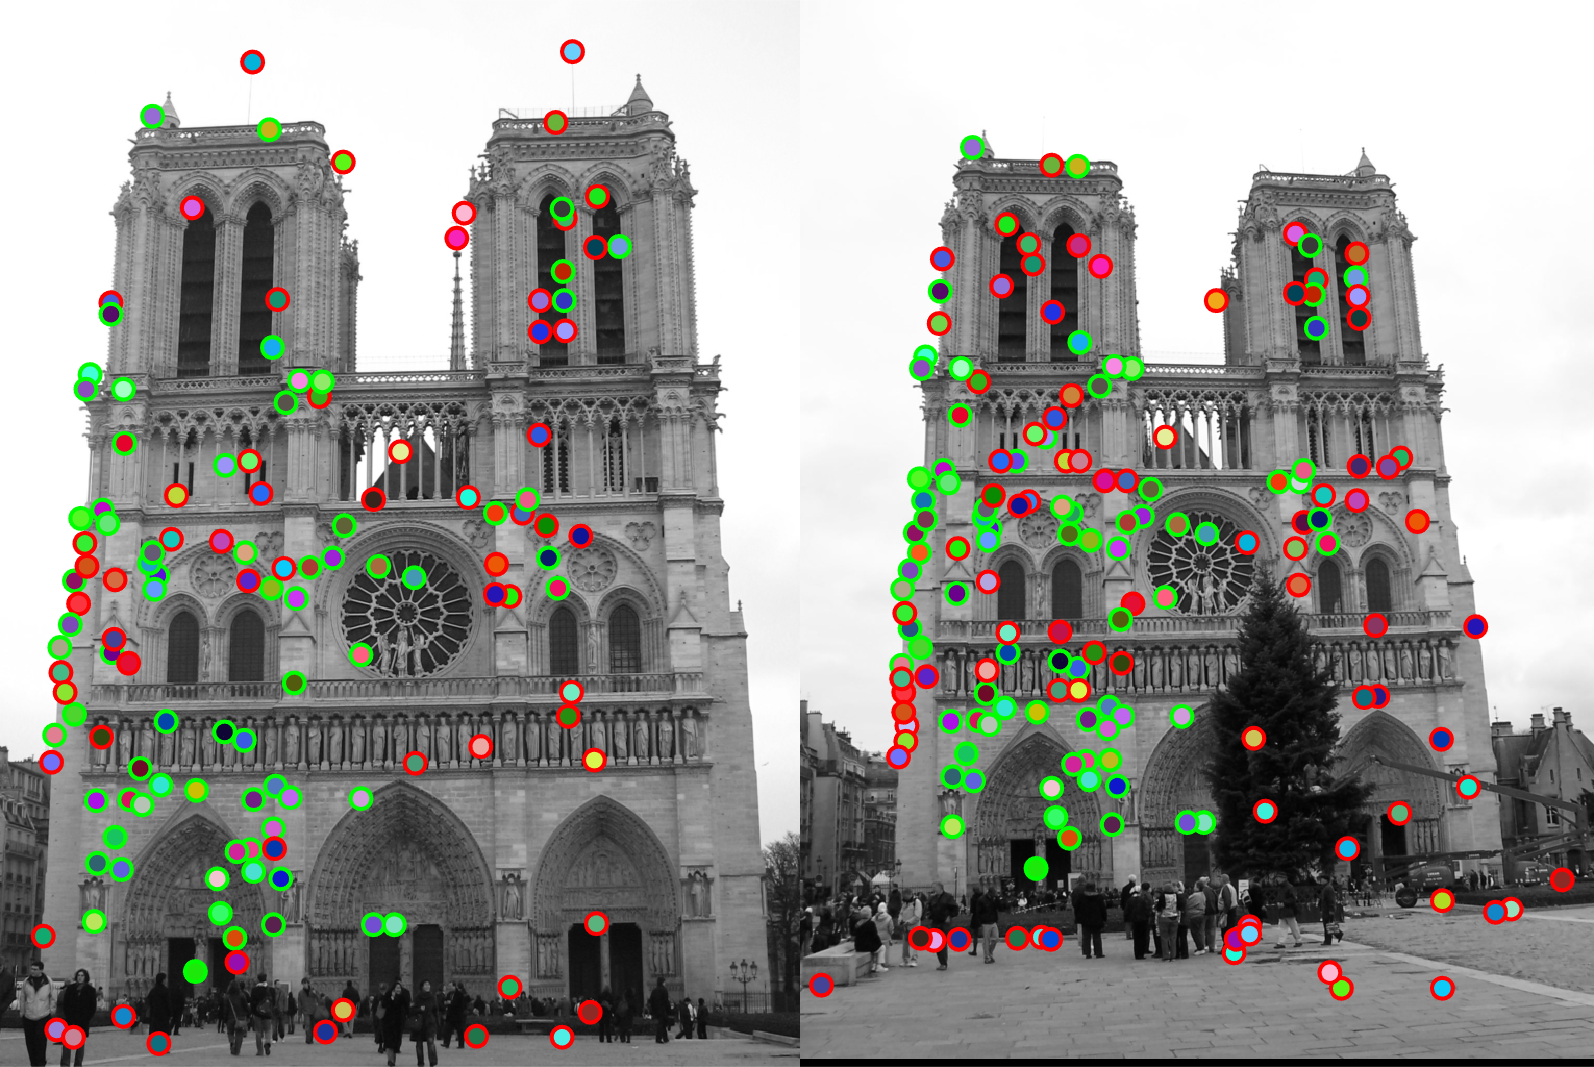
\includegraphics[width=10cm]{writeup/eval_ND bad.png}
    \caption{Notre Dame de Paris (NP)}
    \label{fig:result1}
\end{figure}

\begin{figure}[h]
    \centering
    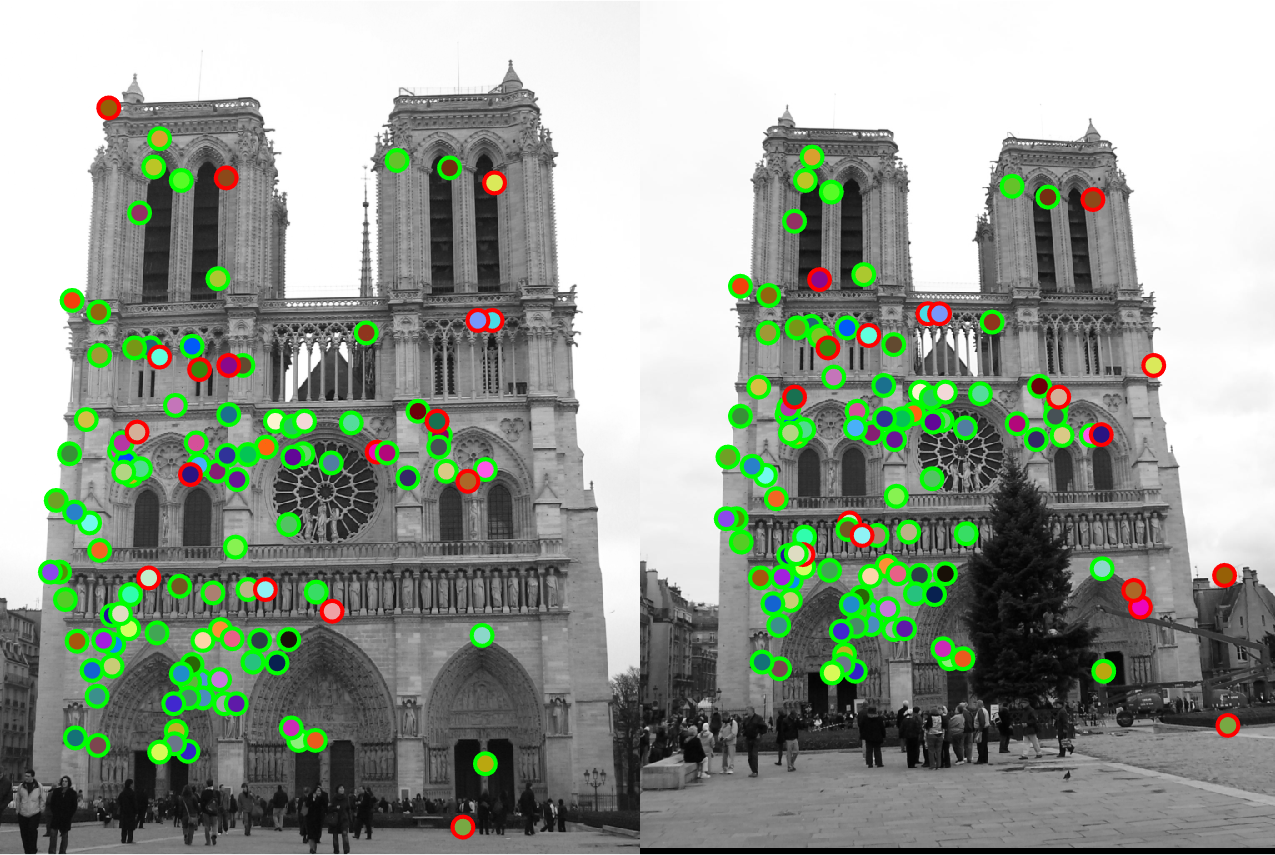
\includegraphics[width=10cm]{writeup/eval_ND.png}
    \caption{Notre Dame de Paris (SIFT-like)}
    \label{fig:result4}
\end{figure}

\begin{figure}[h]
    \centering
    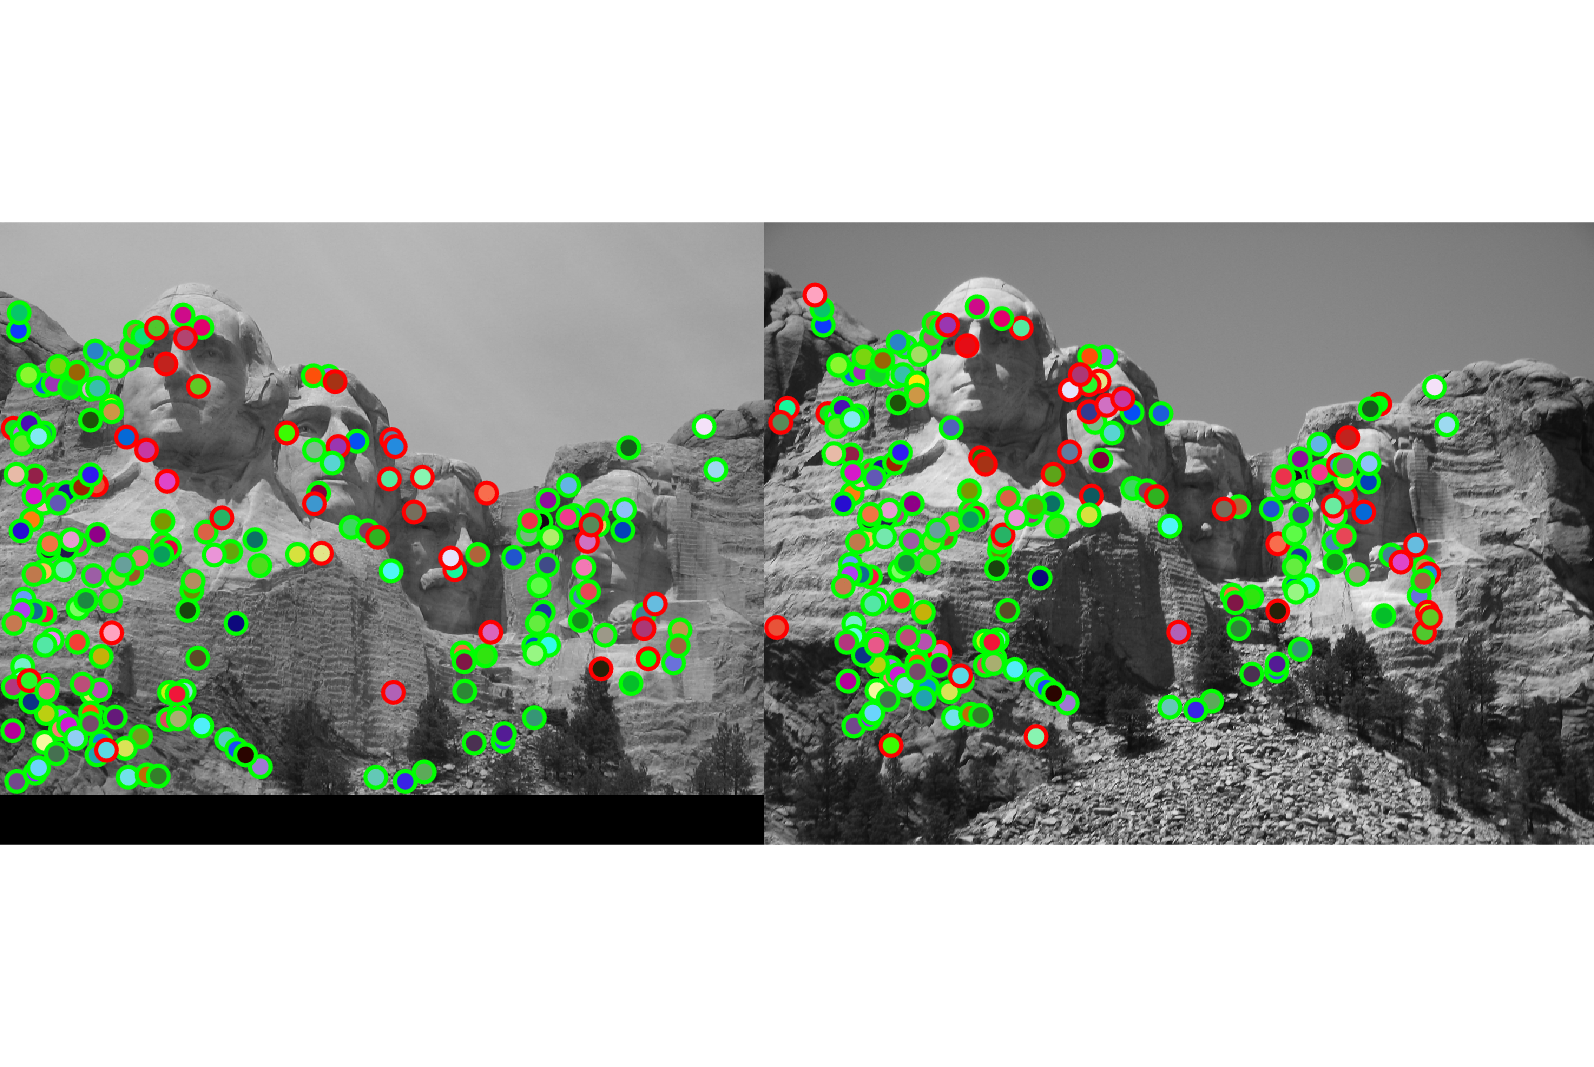
\includegraphics[width=10cm]{writeup/eval_MR bad.png}
    \caption{Mount Rushmore (NP)}
    \label{fig:result2}
\end{figure}
\begin{figure}[h]
    \centering
    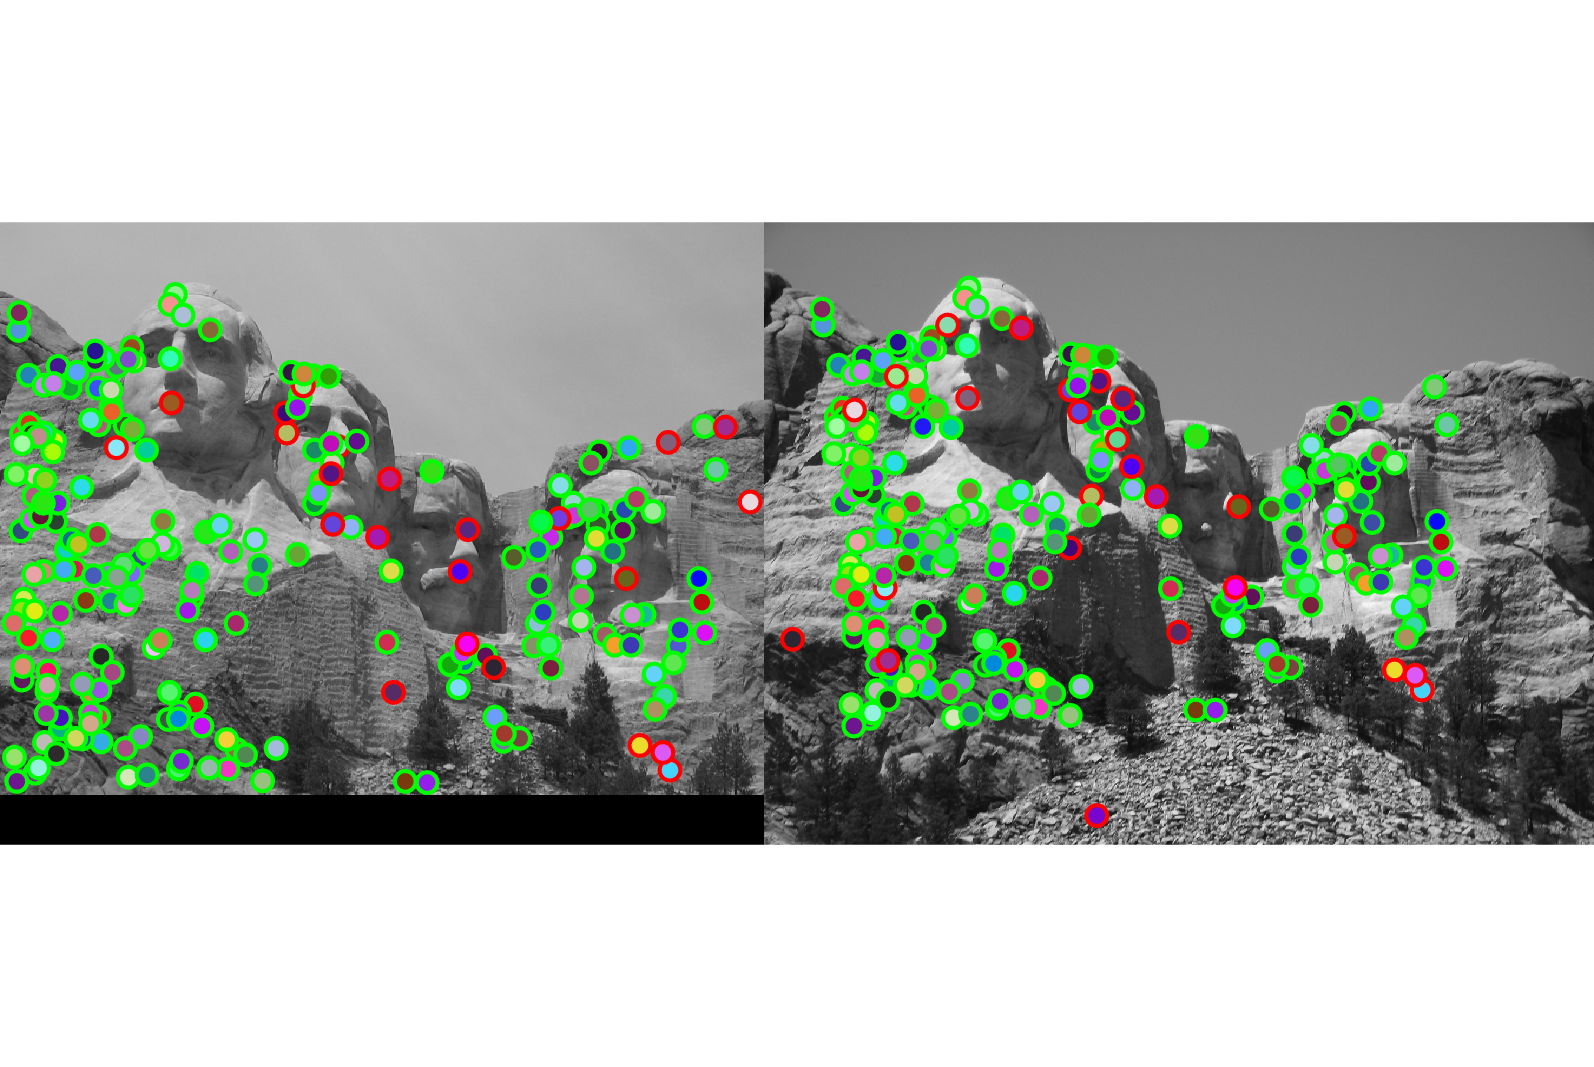
\includegraphics[width=10cm]{writeup/eval_MR.png}
    \caption{Mount Rushmore (SIFT-like)}
    \label{fig:result5}
\end{figure}

\begin{figure}[h]
    \centering
    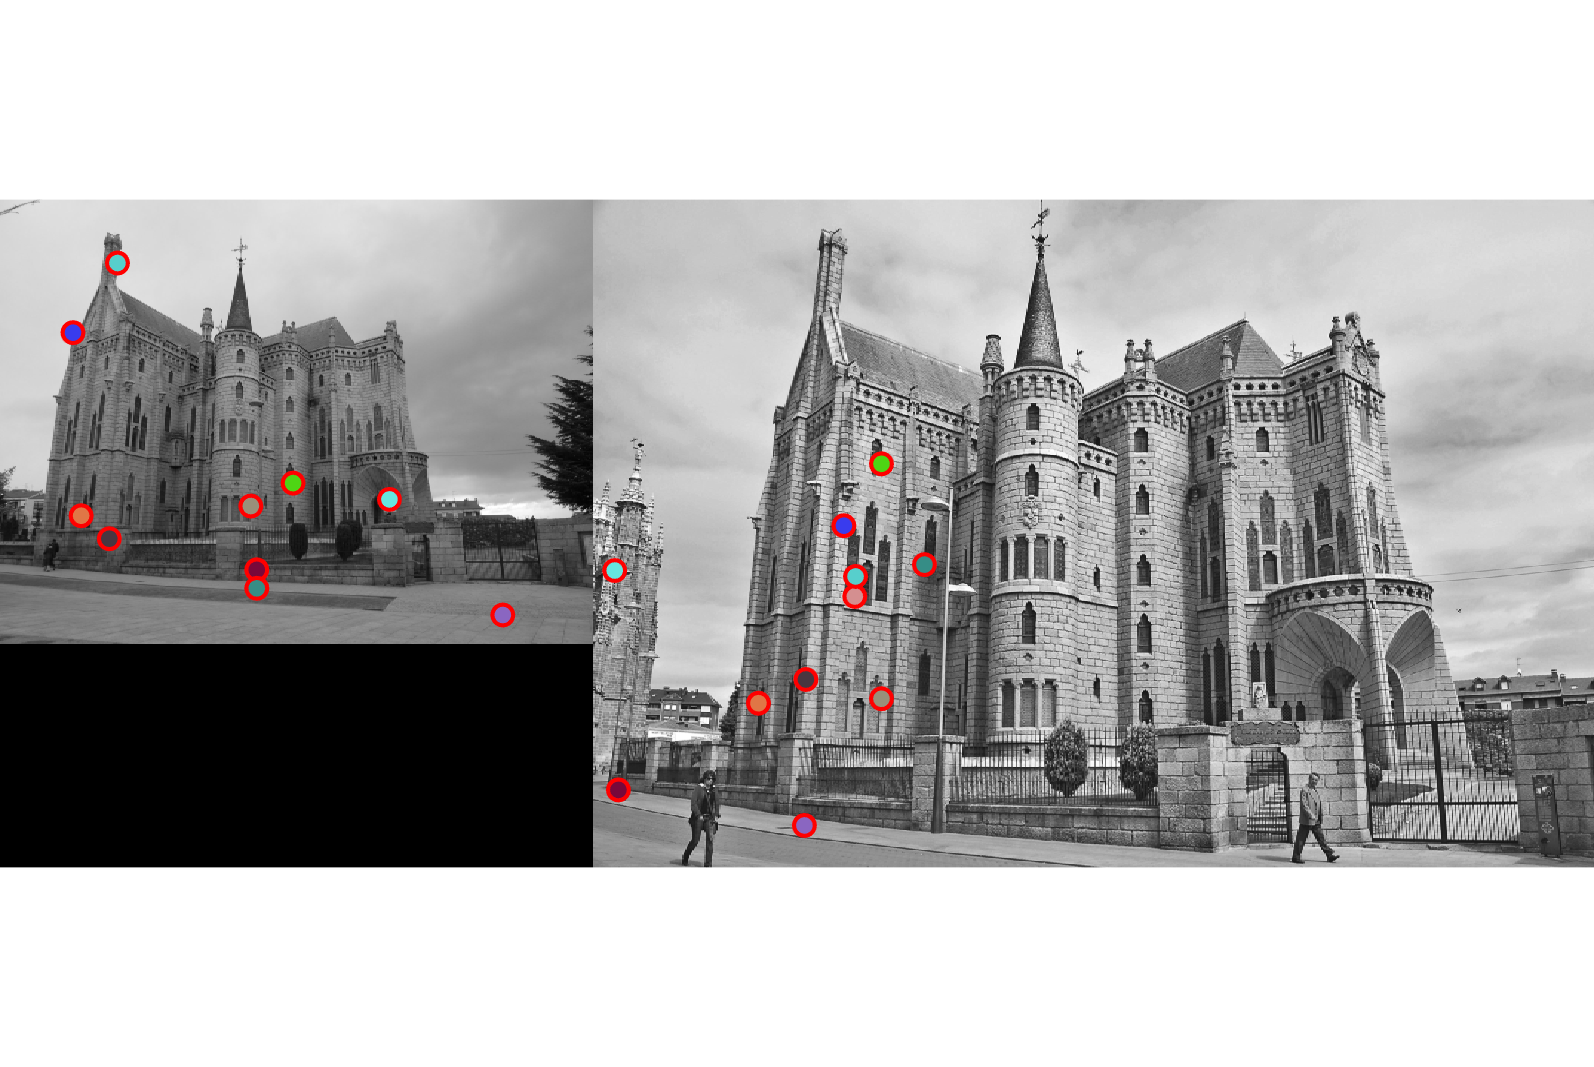
\includegraphics[width=10cm]{writeup/eval_EG bad.png}
    \caption{Gaudi's Episcopal Palace (NP)}
    \label{fig:result3}
\end{figure}

\begin{figure}[h]
    \centering
    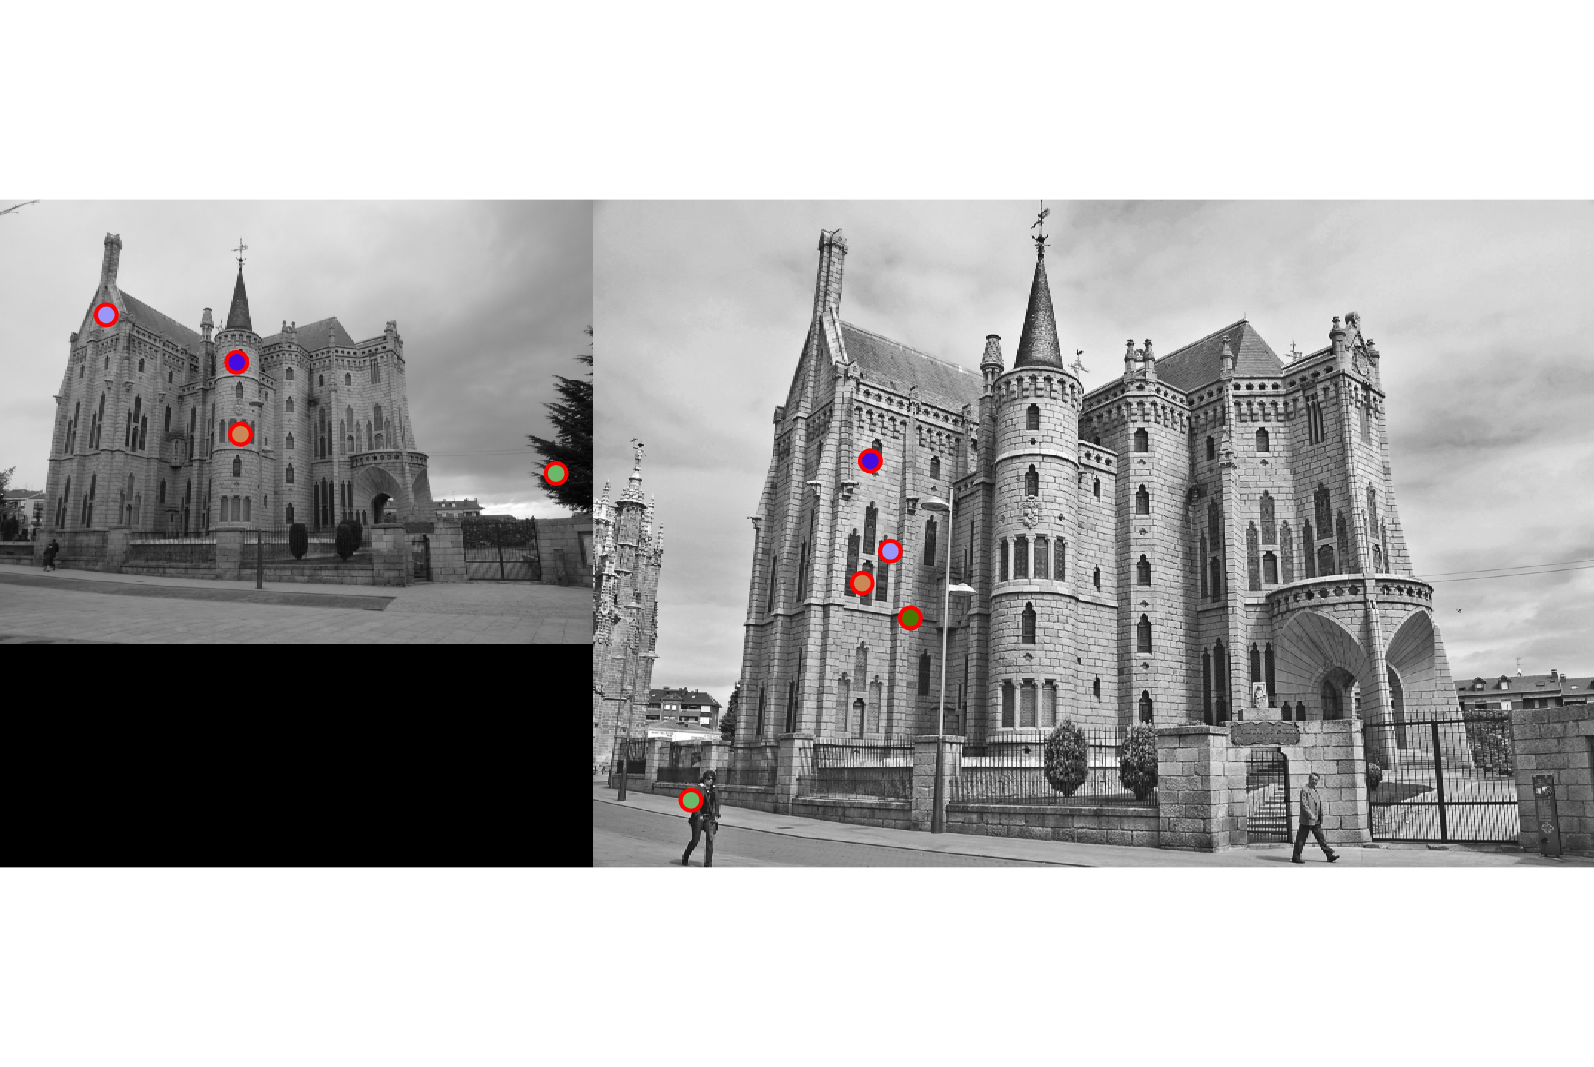
\includegraphics[width=10cm]{writeup/eval_EG.png}
    \caption{Gaudi's Episcopal Palace (SIFT-like)}
    \label{fig:result6}
\end{figure}

\begin{figure}[h]
    \centering
    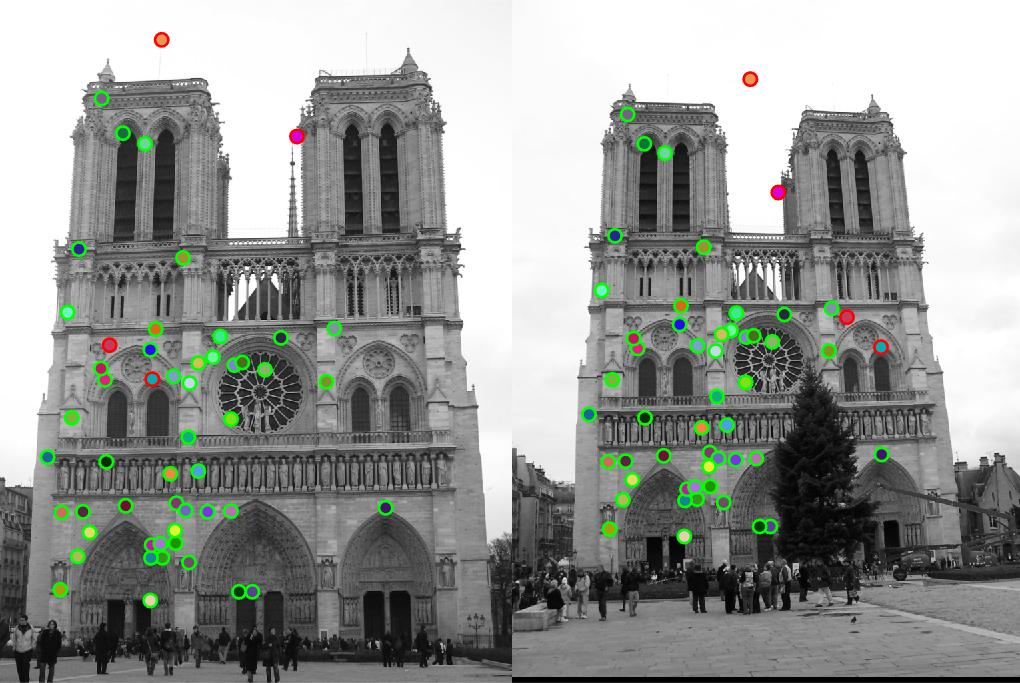
\includegraphics[width=10cm]{writeup/eval_ND without G.jpg}
    \caption{Notre Dame de Paris (SIFT-like) without G()}
    \label{fig:result7}
\end{figure}

\begin{figure}[h]
    \centering
    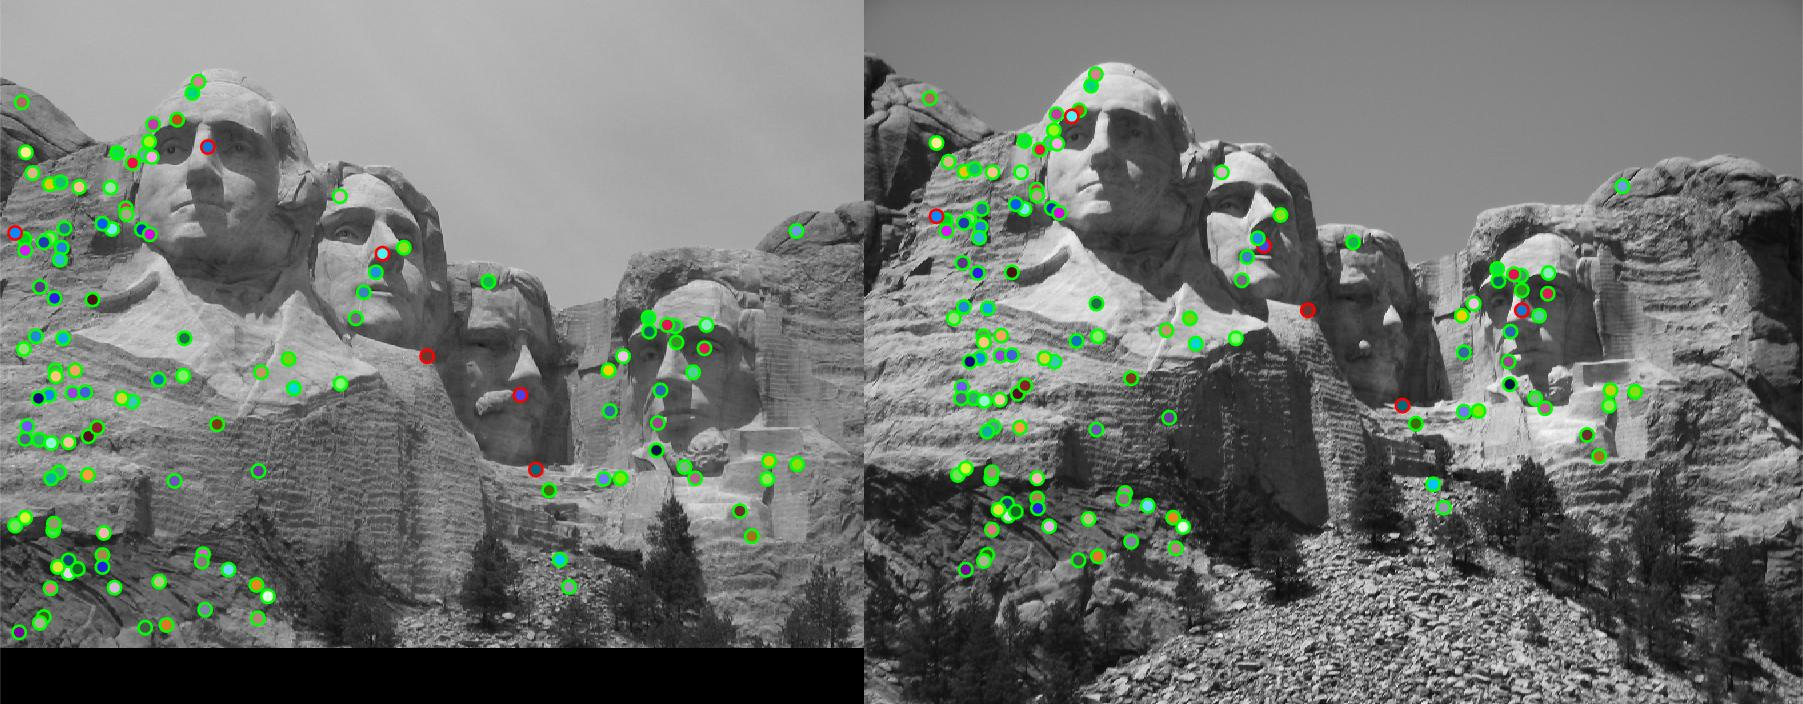
\includegraphics[width=10cm]{writeup/eval_MR without G.jpg}
    \caption{Mount Rushmore (SIFT-like) without G()}
    \label{fig:result8}
\end{figure}

\begin{figure}[h]
    \centering
    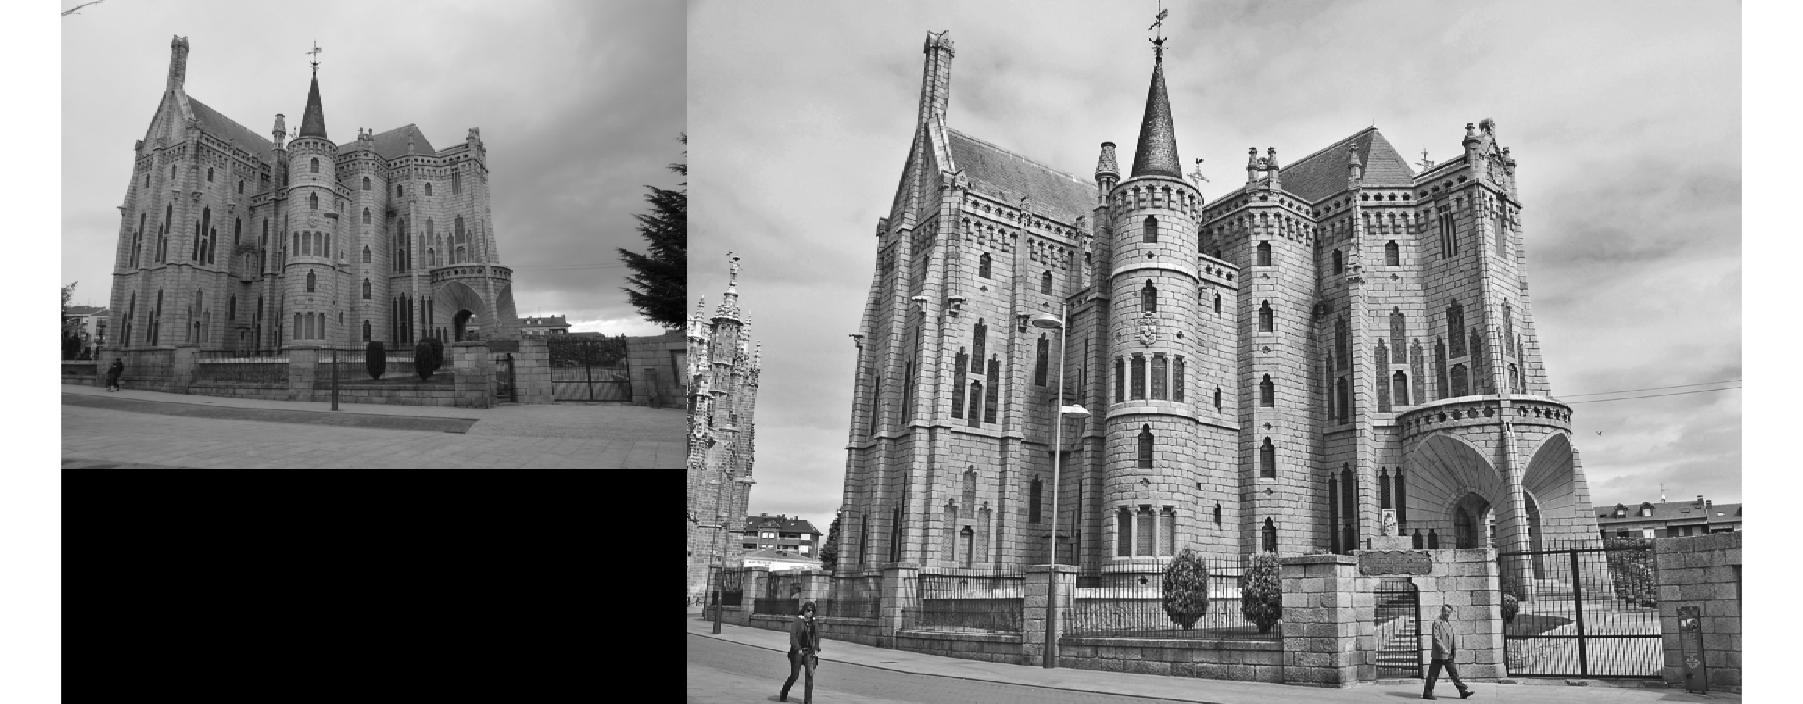
\includegraphics[width=10cm]{writeup/eval_EG without G.jpg}
    \caption{Gaudi's Episcopal Palace (SIFT-like) without G()}
    \label{fig:result9}
\end{figure}

\end{document}
